\documentclass{article}
\usepackage[UTF8]{ctex}
\usepackage{amsmath,amssymb,amsfonts}  % For math symbols and fonts
\usepackage{graphicx}                   % For including images
\usepackage{hyperref}                   % For hyperlinks
\usepackage{cite}                       % For citations

\usepackage{algorithm}
\usepackage{algorithmic}

\usepackage{minted}

\usepackage{amsthm}
% Define new theorem-like environments
% Define environments
\theoremstyle{definition} % Non-italicized style
\newtheorem{definition}{Definition}[section]
\newtheorem{exercise}{Exercise}[section]

% Title and author info
\title{InfermonSAGA Dev Report}
\author{Zhang Jinrui\thanks{alternative email:zhangjr1022@mails.jlu.edu.cn} \\ \texttt{jerryzhang40@gmail.com}}

\date{20250124}  % Empty date; optional, you can also specify a date here

\begin{document}

\maketitle

\begin{abstract}
    In this article, the development processes
    and plans are logged.
\end{abstract}

\section{Main Goal}
The inspiration is from
\cite[DragonDungeonRun]{Dragon_Dungeon_Run},
which is a very simple to implement grid base
game.

But I don't want it just to be a vertical
level only game.
But more rather like a open world game,
with systems like "farming", "fighting",
"adventrue" and even some kind of character
"RPG" and "progression".

For the "adventure" part, the world is just
a lot of square grid, which the player is
always takeup one grid.
The grid can be viewed as
little piece of a manifold.
The map of the world can be a lot of
2D-manifold with different inherent
($nP^2$ or $nT^2$, does't mater afterall
we will have a more realistic and
non-theoretical method to realise this in
a game),
connected by "portal". This forms the
core "adventrue" part of the game.

For the "fighting" part is just like
usual RPG game, the monster or enemies also
takeup one square grid, and less dynamic
are needed for the moster AI.

For the "farming" part we can use the
tools to make a square grid in to a
farmland,which we can grow agricultures
on this square grid.
The productions by farming can help
"exploration" and "fighting"

The final part is mainly need high
quality character design. This need
a lot of art and game script effort,
which may not be affordable for myself
at present.

\section{Roadmap}
\subsection[adventrue]{Topology structure for adventrue}
For this we need a mathematic based
data structure to save our map and
portals.

Take the one eighth of a sphere as an example.
Figure~\ref{fig:sphere} shows how this expansion
will look in general.

\begin{figure}[!ht]
    \centering
    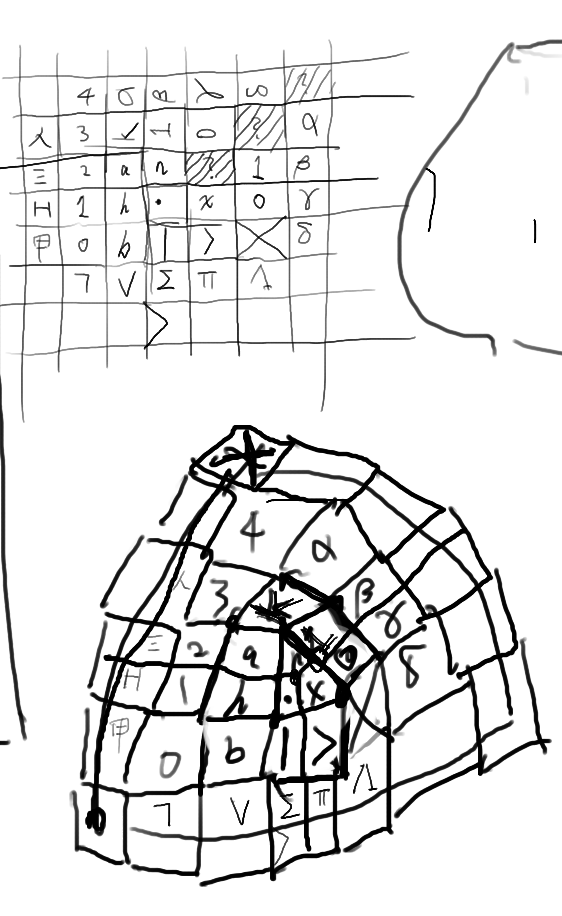
\includegraphics[width=0.45\textwidth]{figs/generalExplanation.png}
    \caption{Suqare tile expansion of $\frac{1}{8}$ sphere}
    \label{fig:sphere}
\end{figure}

The shadow area with a question mark,
means this place have a conflict and
will be view as a "Portal".

\begin{definition}[Portal]
    \label{def:Portal}
    The shadowed question marked tile
    is a portal.
\end{definition}

This is inevitable because the curvature
of the sphere is not equal to the plane.
But this is a flavor of the Infermon view
the world he lived in.
When you try to enter the "portal" you will end
in an another square the current square
you leave connected to.

The second example is about a important operation
to manipulate of the space Topology.
Which is Tunneling.
This process is showed in
Figure~\ref{fig:Tunneling}.
In this process, tile "A" was turned into a
portal tile.

\begin{figure}[!ht]
    \centering
    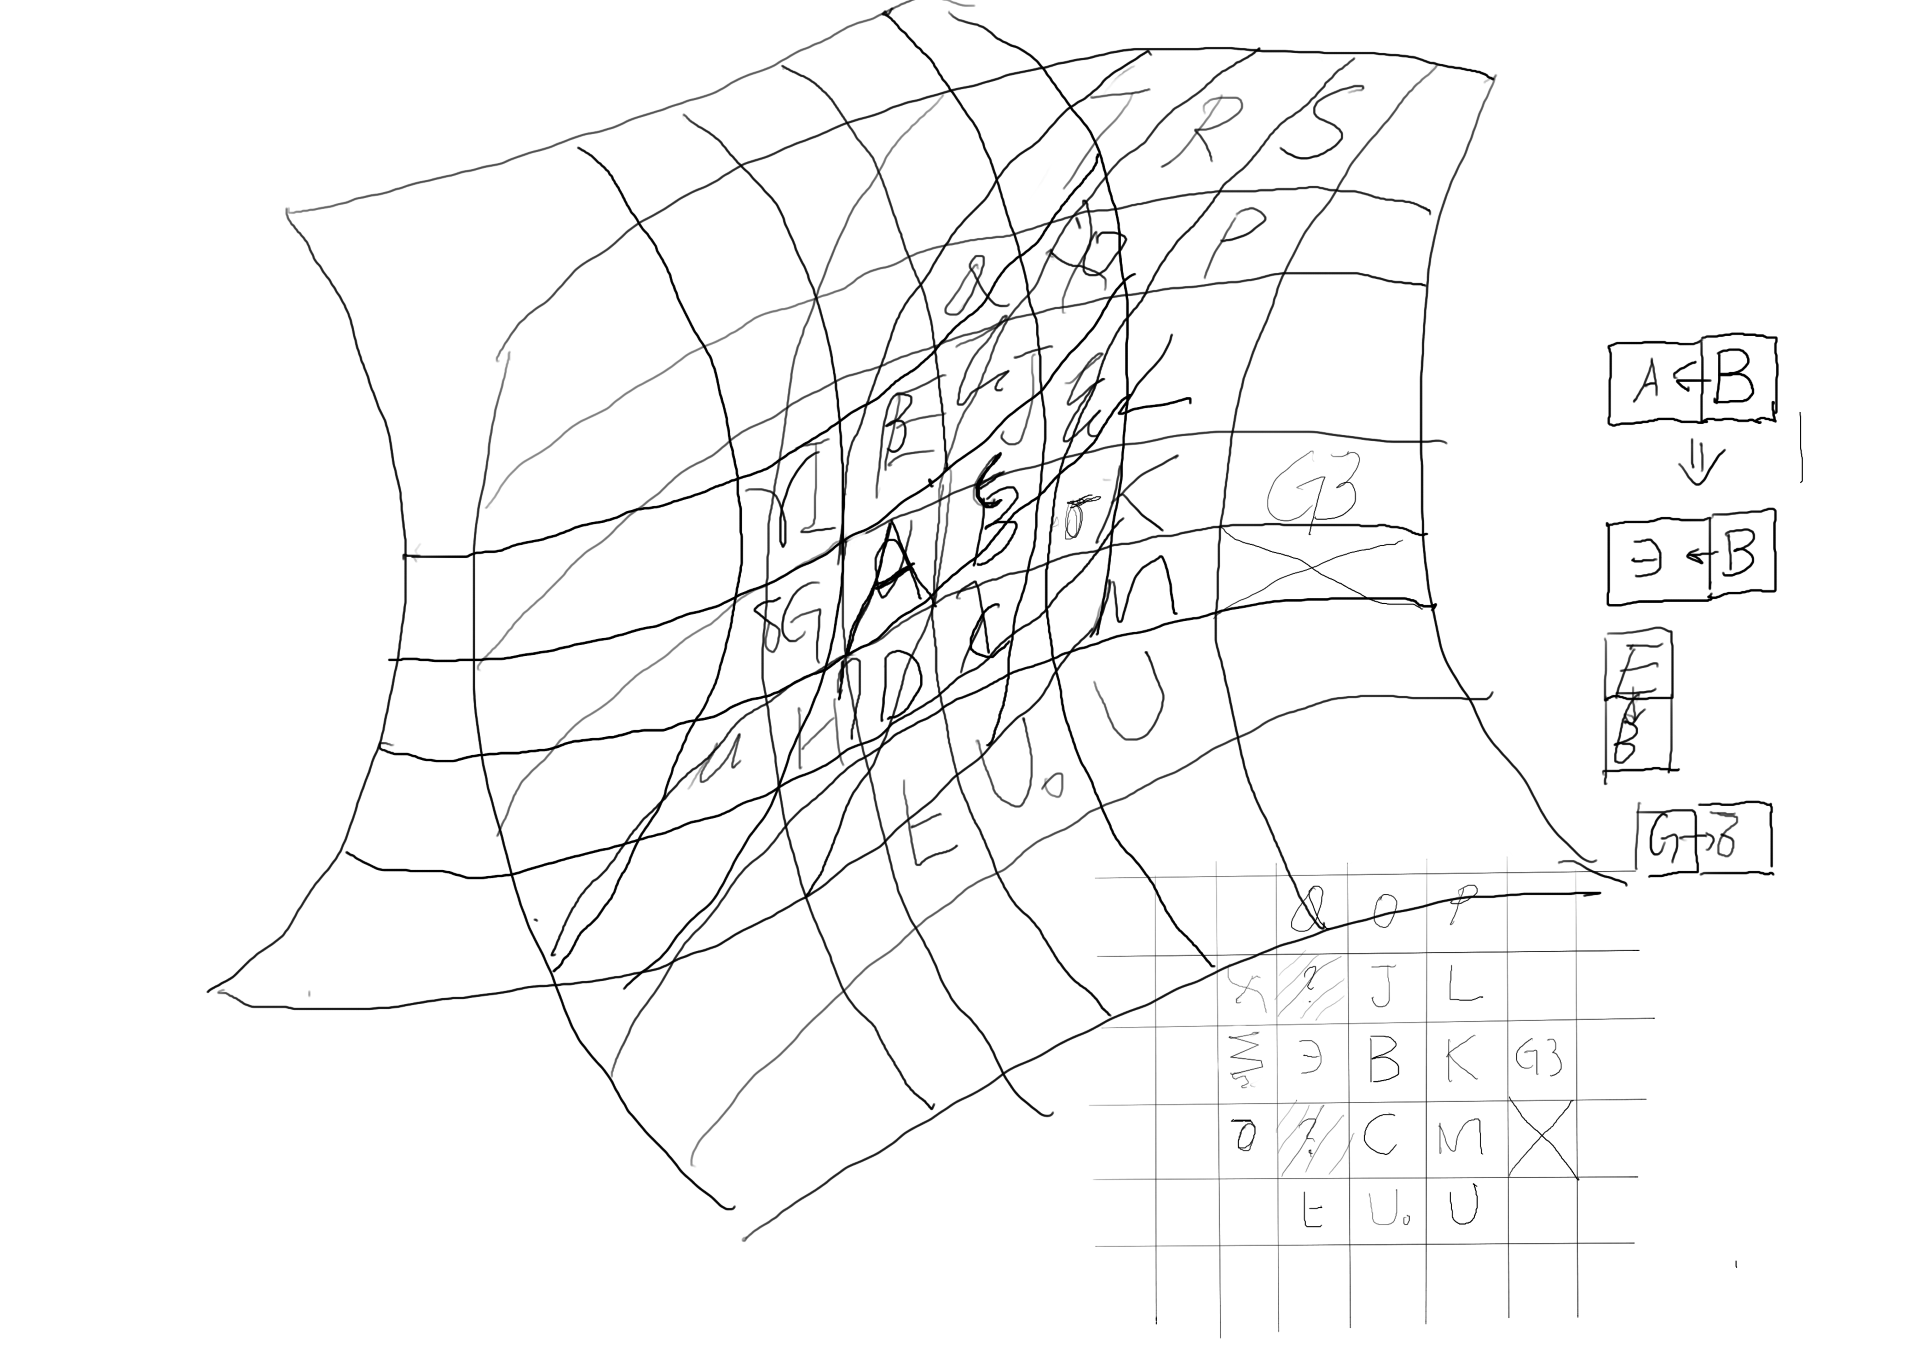
\includegraphics[width=0.45\textwidth]{figs/tunneling Portal.png}
    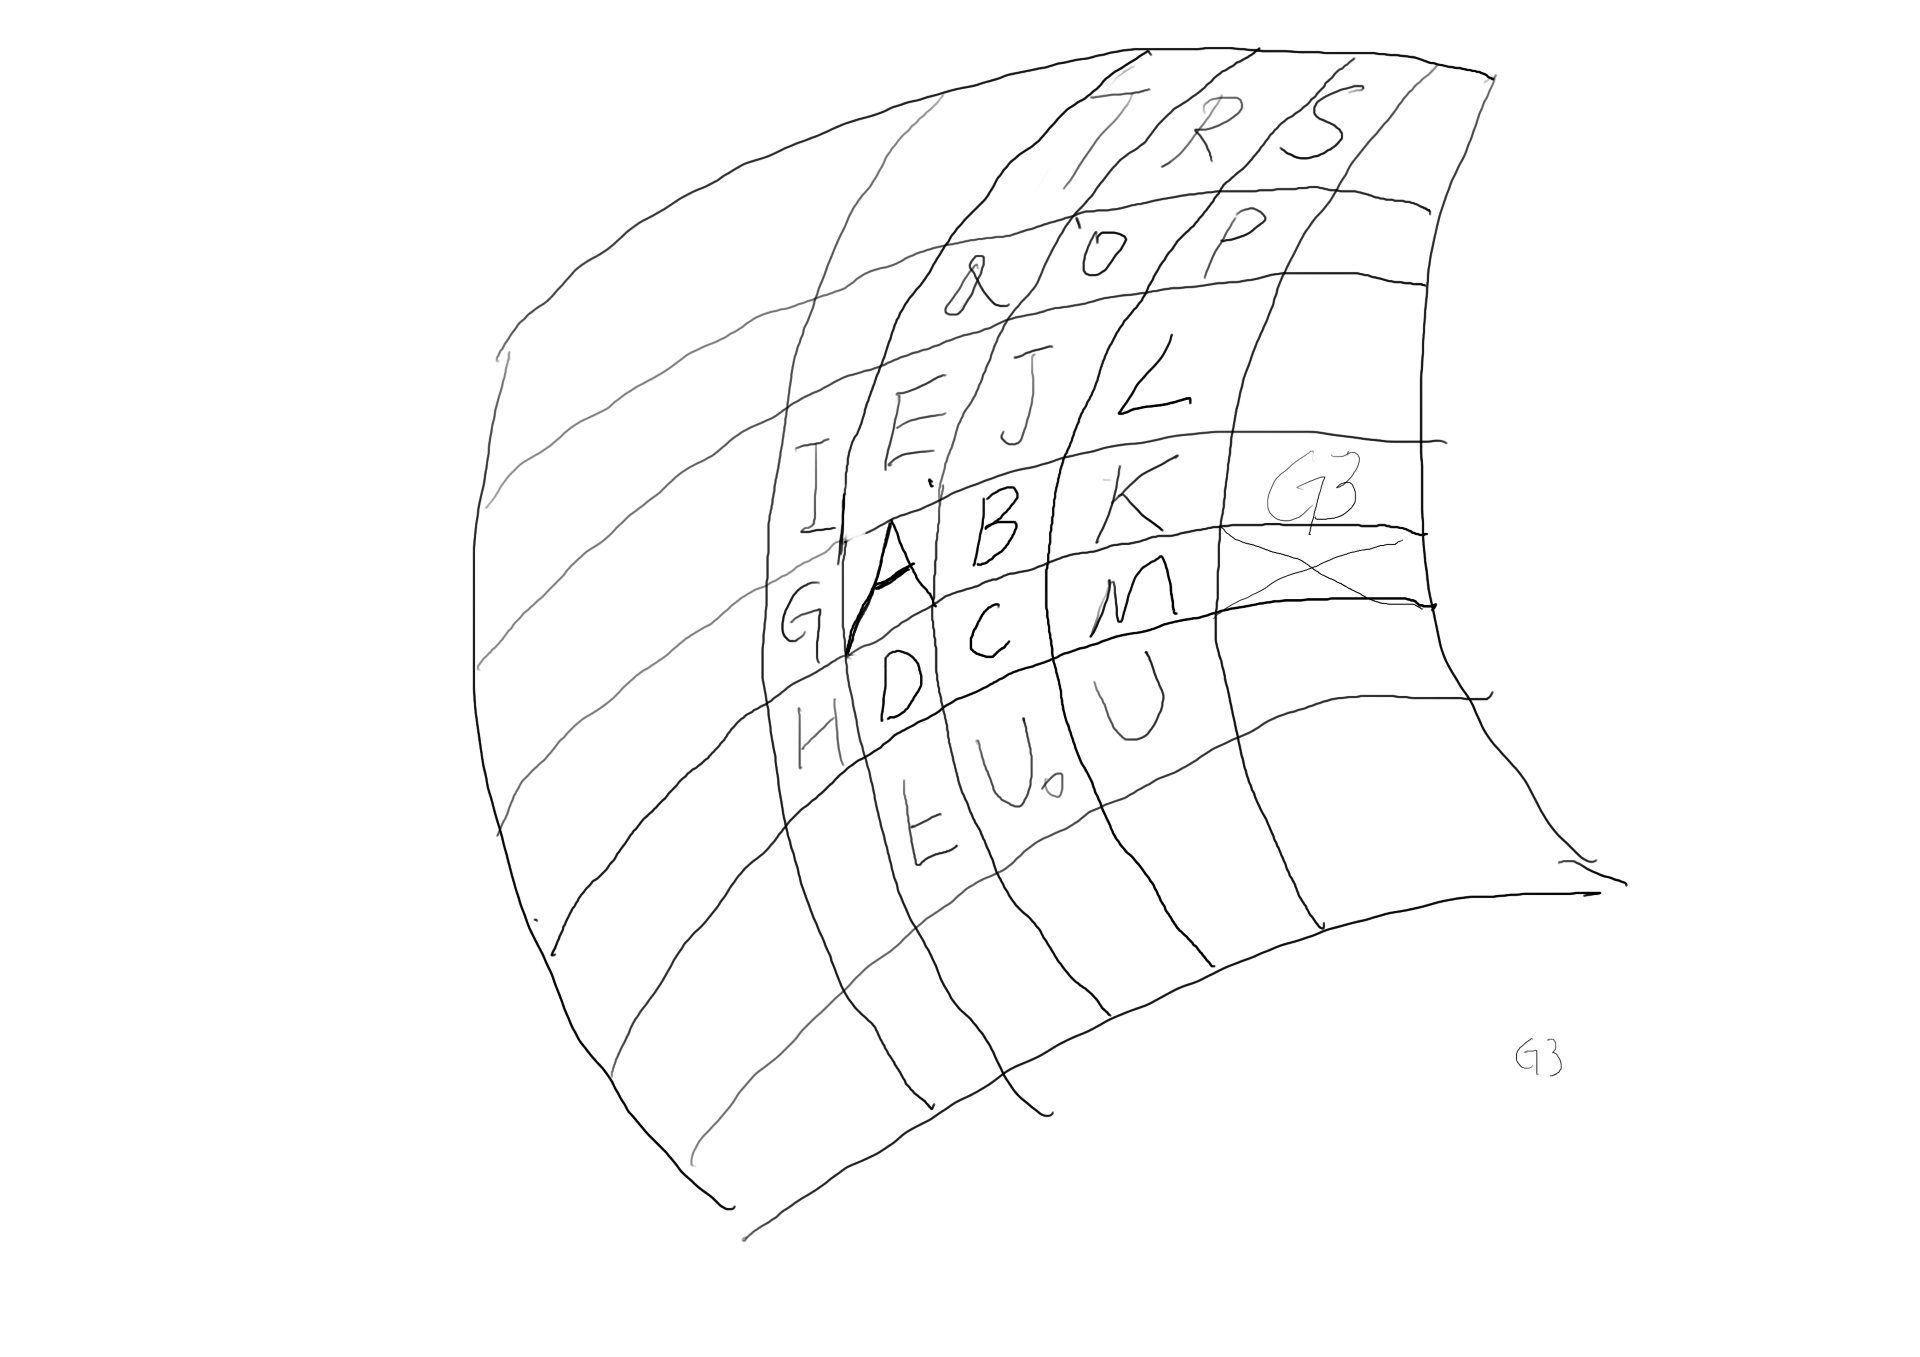
\includegraphics[width=0.45\textwidth]{figs/tunneling Portal0.png}
    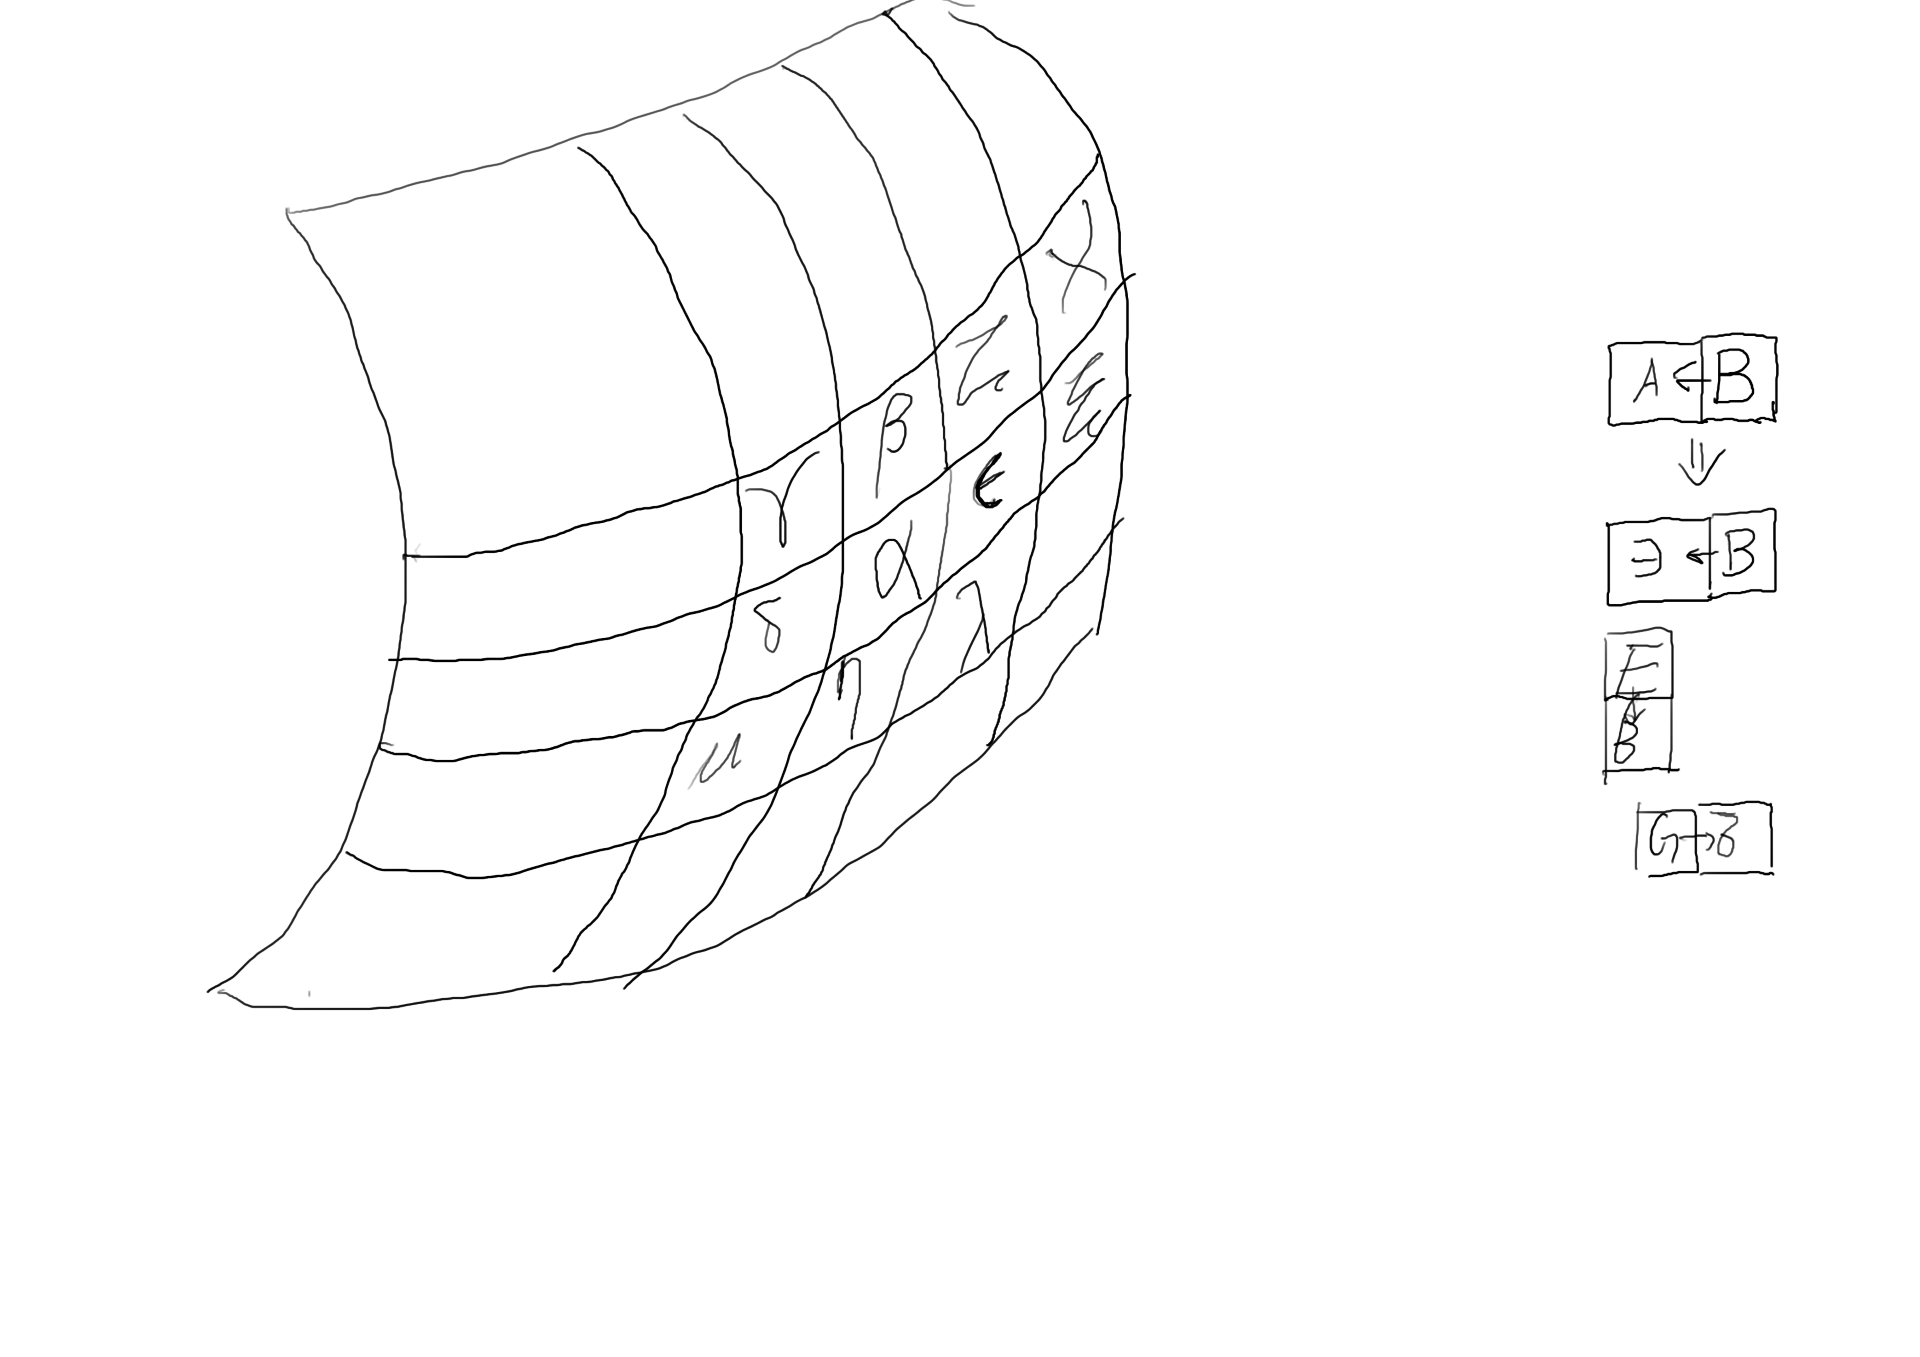
\includegraphics[width=0.45\textwidth]{figs/tunneling Portal1.png}
    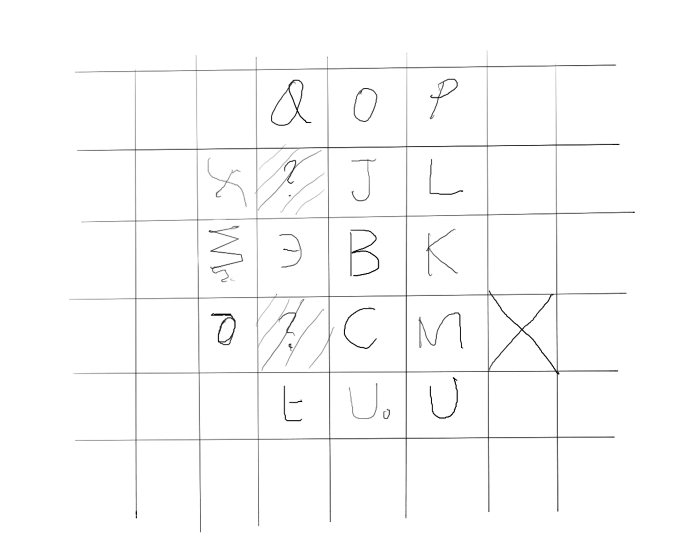
\includegraphics[width=0.45\textwidth]{figs/tunneling Portal tiling.png}
    \caption{Tunneling process}
    \label{fig:Tunneling}
\end{figure}

For there is some special case for the portal,
which is the Tunneling portal,
we need to make some more definition.
The Tunneling portal has a different visualizaiton
requirement.

\begin{definition}[Intrinsic Portal]
    \label{def:IntrinsicPortal}
    Those portal that inevitable to create,
    when using the ordinary way to expand
    the Suqare tilling.
\end{definition}

\begin{definition}[Artificial Portal]
    \label{def:ArtificialPortal}
    Those portal that made by the Tunneling
    process, surround by a 8-tile valid loop.
\end{definition}

The whole world is just a single map,
the map is maintained in a single list.
But the world can be a several disconnected,
space bubble.

A block should save four adjacent block.
When render it to a Square tile expansion to
a 2d-gird. inevitablly some Intrinsic Portal
will be created.

Another Portal type is ArtificialPortal which
treat as a object on a space block.
The ArtificialPortal have linked two space block
together, and if one goes into one from
one side, he will come out in the conjugate
space block from the other side.

Tunneling process is a advanced technique,
for the player have some extra level in the
game, he would be modify the link of the adjacent
relationship of a single block.

Now we will be focous to realise this data
structure

\subsubsection[list]{list}
The following is a implementation GPT give.
This list is for save the map data in a
linked list. The Suqare tile block is save
in the list.
\begin{minted}[frame=single, linenos]{cpp}
#include <iostream>
#include <list>
#include <memory>
#include <fstream>
#include <string>

template <typename T>
class MyList {
private:
    std::list<std::unique_ptr<T>> elements;

public:
    // 添加元素
    void push_back(std::unique_ptr<T> element) {
        elements.push_back(std::move(element));
    }

    // 删除第一个元素
    void pop_front() {
        if (!elements.empty()) {
            elements.pop_front();
        }
    }

    // 遍历并打印元素
    void print_all() const {
        for (const auto& element : elements) {
            element->print();
        }
    }

    // 保存到文件
    void save_to_file(const std::string& filename) const {
        std::ofstream outFile(filename);
        if (!outFile) {
            std::cerr << "Error opening file for writing." << std::endl;
            return;
        }

        for (const auto& element : elements) {
            outFile << *element << std::endl;
        }

        std::cout << "List saved to file: " << filename << std::endl;
    }

    // 从文件加载
    void load_from_file(const std::string& filename) {
        std::ifstream inFile(filename);
        if (!inFile) {
            std::cerr << "Error opening file for reading." << std::endl;
            return;
        }

        elements.clear(); // 清空当前链表
        while (!inFile.eof()) {
            auto element = std::make_unique<T>();
            if (inFile >> *element) {
                elements.push_back(std::move(element));
            }
        }

        std::cout << "List loaded from file: " << filename << std::endl;
    }
};

// 示例数据结构
struct DataBlock {
    int id;
    std::string name;

    DataBlock() = default;
    DataBlock(int id, const std::string& name) : id(id), name(name) {}

    void print() const {
        std::cout << "ID: " << id << ", Name: " << name << std::endl;
    }

    // 序列化到文件
    friend std::ostream& operator<<(std::ostream& os, const DataBlock& block) {
        os << block.id << " " << block.name;
        return os;
    }

    // 从文件反序列化
    friend std::istream& operator>>(std::istream& is, DataBlock& block) {
        is >> block.id >> block.name;
        return is;
    }
};

int main() {
    MyList<DataBlock> myList;

    // 添加元素
    myList.push_back(std::make_unique<DataBlock>(1, "Block1"));
    myList.push_back(std::make_unique<DataBlock>(2, "Block2"));

    // 打印链表
    std::cout << "Initial list:" << std::endl;
    myList.print_all();

    // 保存到文件
    myList.save_to_file("data.txt");

    // 从文件加载
    myList.load_from_file("data.txt");

    // 打印加载后的链表
    std::cout << "After loading from file:" << std::endl;
    myList.print_all();

    return 0;
}
\end{minted}

\subsubsection[tile]{Square tile}


\subsection[fighting]{fighting system}
\subsection[farming]{farming system}

\section[deps]{Dependencies}
This section, the third-party dependencies
will be logged and explained about how they
are used in this specific project.
\subsection[GLAD]{GLAD}
The glad is used for the version that support
the multiple-window graphics. The configuration
for this dependence is according to
\cite[gladMultiwinMx]{GLAD_multiwin_mx}. We
need to do this once in the top CMakeLists.txt.

\begin{minted}[frame=single, linenos]{cmake}
    set(GLAD_SOURCES_DIR "${PROJECT_SOURCE_DIR}/glad")
    add_subdirectory("${GLAD_SOURCES_DIR}/cmake" glad_cmake)
    glad_add_library(glad REPRODUCIBLE MX API gl:core=4.3)
\end{minted}

Remember to include glad right before glfw as
follow.

\begin{minted}[frame=single, linenos]{cpp}
    #include <glad/gl.h>
    #include <GLFW/glfw3.h>
\end{minted}

\subsection[GLFW]{GLFW}
The main graphics dependencies is glfw3.
I used its sources code form its Github
repository.

And Simply use this two line in CMakeLists.txt
is okay.

\begin{minted}[frame=single, linenos]{cmake}
    add_subdirectory(glfw)
    include_directories(glfw/include)
\end{minted}

Then include GLFW in the file use it.

\begin{minted}[frame=single, linenos]{cpp}
    #include <GLFW/glfw3.h>
\end{minted}

\subsection[IMGUI]{IMGUI}
I choose to use the maximum features of the
imgui, which contains "docking" and
"Multi Viewports"

To set up imgui with the glad and glfw is
according to
\cite[setupImgui]{example-if-you-are-using-glfw--openglwebgl}.

To set up imgui with "Multi Viewports" feature
is according to
\cite[text]{Multi-Viewports}.


% \section{Current Roadmap}
% \subsection{statistics}
% \subsubsection{X is Close Price}
% Choose $X=\mathbb{R}$ which is the close price.
% \subsubsection{X is the difference between MA and close price}
% By intuition, when the price is above the MA,
% It should some how comes back, and vice versa.
% \subsection{machine learning}
% \subsubsection{X is prefix sequence}
% To find feature in the prefix sequence. The
% Transformer and 1D-CNN is now under
% the consideration.
% This topic derives experiments including
% EXP20250119

% \section{EXP20250119 prefix sequence}
% This experiment use the prefix sequence
% to be the condition space X.

% \begin{definition}[prefix space]
%     All possible prefix sequence form a space X
% \end{definition}

% If the market is EMH.
% By Definition~\ref{def:mydefinition}, this means
% for all subset of $X$,
% $\mathbb{E}_{W\mid A}(W)\doteq 0$. That is
% $
%     \forall A\subseteq X,
%     \mathbb{E}_{W\mid A}(W)\doteq 0
% $

% So if we want to find the vulnerability of
% the market we want to find a $X$ such that
% there exist a $A\subseteq X$ agrees that
% $\mathbb{E}_{W\mid A}(W)>0$

% Consider a simplest senario, that is, we only
% treat the sequence as descend and ascend. Then
% for a space of length $L$ then
% $\left|X\right|=2^L$, which is a nightmare for
% statistics, so I'm forced to use machine learning
% to try to find something.

% \subsection{Data regularization}
% Current data regularization is as follow.
% Suppose we have a time series
% $P_t \in \mathbb{R}_+$
% We want it range from $(0,1)$ and have a symmetry
% about descend and ascend around zero.
% So let $Lr_t=\ln(\frac{P_{t+1}}{P_{t}})$.
% $Lr_t\in \mathbb{R}$ and then
% $Sg_t=\tanh(Lr_t)$

% Then $X=\{(Sg_k)|t_{start}\leq k\leq t_{end}\}$

% \subsection{Conclusion}
% In \cite[PrefixSequence]{EXP20250119PrefixSequence}
% I implemented the function to get $Sg_t$

% The first Stage experiment result is
% very bad in \cite[Cov1d]{EXP20250119PrefixSequenceGPTCov1d}

% \section{EXP20250120 MA}
% This experiment use the difference between
% MA and close price as the space X.

% \begin{definition}[MACP difference]
%     $D_t^N:=A_t^N-P_t$
%     which
%     $A_t^N=\sum_{k=t-N+1}^tP_k$
%     which $N$ is a hyper-parameter
%     when N is a single number then $D_t:=D_t^N$
%     is a time series of number
%     when $N$ can be multiple different numbers
%     then $D_t^N$is a vector time series.
% \end{definition}

% \subsection[Fix N]{Fix $N$}
% Suppose $N$ is a fixed single number then
% $D_t$ is a time serie.
% To simplify the problem we define a
% classification variable $V$
% \begin{definition}[Ternary Classification]
%     $
%         V_t:=
%         \begin{cases}
%             1,  & P_t\in\left(0.1,+\infty\right)  \\
%             0,  & P_t\in\left(-0.1,0.1\right)     \\
%             -1, & P_t\in\left(-\infty,-0.1\right) \\
%         \end{cases}
%     $
% \end{definition}

% Use the bin size of $0.01$ which is the smallest
% increment of the price. Do the statistics over
% all $D_t\in\mathbb{R}$ with the bin size $0.01$
% to obtain the conditional probability distribution
% of the random variable $V_t$

% \subsection{Result}
% \begin{figure}[h!]
%     \centering
%     \includegraphics[width=0.45\textwidth]{figs/EXP20250120MA/EXP20250120MA_RandomWalk.png}
%     \includegraphics[width=0.5\textwidth]{figs/EXP20250120MA/EXP20250120MA_PRICE.png}
%     \caption{RandomWalk(left),realdata(right)}
% \end{figure}
% The result shows for the Random RandomWalk, the
% curve is like sigmoid but exchude a normal
% distribution for $V_t=0$
% While the distribution for realdata is more
% intricate the blue curve is more like a
% t-distribution.
% \begin{figure}[h!]
%     \centering
%     \includegraphics[width=0.45\textwidth]{figs/EXP20250120MA/EXP20250120MA_Prc.png}
%     \includegraphics[width=0.5\textwidth]{figs/EXP20250120MA/EXP20250120MA_Prc_.png}
%     \caption{Fixed:RandomWalk(left),realdata(right)}
% \end{figure}

% The original code that GPT write, use $D_{t+1}$
% to predict $V_t$ which in the RandomWalk shows
% significantly distribution bias.This fixed version
% has test on the RandomWalk don't have any bias
% on the RandomWalk.


% \section{Methodology}
% \subsection{first approach}
% The first idea is simple. For a one-variable function $u(t)$,
% define a second-order differential equation
% in its general form $(\forall t)(F(\frac{d^2u}{{du}^2},\frac{du}{dt},u)=0)$.

% The data of the function $u(t)$ are given in tuples denote as
% $(T,U)_i\equiv(T_i,U_i)$. And it is natural to denote the differentials
% by $U^{t}_{i}$ and $U^{tt}_{i}$. There are several methods to compute
% these two differentials, including just using the definition of
% the derivative. In this article, local PCA are compute to obtain
% these differentials. Local PCA means finding the nearest K neighbors
% of a given point, which K is a hyper parameter, and performing PCA
% on these points close to each other to get the principal direction.
% The slope of this direction is the derivative $U^{t}$ in general.
% Repeat this process on $(T,U^{t})$ to obtain $U^{tt}$

% Create a FCN denote as $f$ to represent
% $F(\frac{d^2u}{{du}^2},\frac{du}{dt},u)$
% $F$ to be $0$ at every data points and to be $1$ all elsewhere is wanted.

% To achieve these requirements, we evaluate $f$ at all the data points,
% and train the network to evaluate these points to $0$. Then randomly sample
% the points of $\mathbb{R}^{3}$ and train these points to be $1$ Algorithm\ref{algor:1}.


% \begin{algorithm}
%     \caption{$f$ trainer}\label{algor:1}
%     \begin{algorithmic}[1]
%         \REQUIRE Input parameters $f,T_i, U_i, U^{t}_{i}, U^{tt}_{i}$
%         % \ENSURE Output $z$
%         \STATE Initialize $f$ randomly
%         \REPEAT
%         \STATE $F_i \leftarrow f(U_i,U^{t}_{i},U^{tt}_{i})$
%         \STATE $RAND_i \leftarrow$ randomly sample in $\mathbb{R}^{3}$
%         \STATE $R_i \leftarrow f(RAND_i)$
%         \STATE $L \leftarrow meanSquareError(F_i,0)+0.1*meanSquareError(R_i,1)$
%         \STATE back Propagation against $L$ to optimize $f$
%         \UNTIL {$L$ meets requirement}
%         % \FOR{each $i$ from $1$ to $n$}
%         % \ENDFOR
%         \RETURN $f$
%     \end{algorithmic}
% \end{algorithm}

% Once The $f$ was obtained, we can perform PINN as a decoder
% to generate new data.


% The experiment code for the pictures in Results can
% be run by a Python program in Github\cite[deSineTasks]{firstApproachGithubProject}
% The requirement environment may be installed using\cite[reqs]{Envreqs}

% \subsection{approach with linear assumption}
% For a small randomly sampled data set, the data points
% in the differential vector space
% $\left[\begin{matrix}{U}&{U^{t}}&{U^{tt}}\end{matrix}\right]$
% are a low-dimensional manifold. With only one equation to satisfy, the dimension of the manifold in the latent space would be exactly one less than the whole space dimension. In the second-order
% differential equation case, the manifold has to be a two-dimensional
% manifold. As the pictures show in Figure\ref{one:dimensionalmani},
% if we only have some of the experimental data input, with
% the algorithm in the first approach, we would set all the
% values in the one-dimensional manifold to $0$ but all elsewhere
% to $0$ which is only one specify solution with the same
% initial condition as the input data.
% % \begin{figure}[ht!]
% %     \centering
% %     \includegraphics[width=1.0\textwidth]{figLinearSine1_cbf0039b/draw_3d.png}
% %     \caption{vectors $\left[\begin{matrix}{U}&{U^{t}}&{U^{tt}}\end{matrix}\right]$ sit on 1-dimensional manifold}
% %     \label{one:dimensionalmani}
% % \end{figure}

% To have more generalization ability, sacrifice
% is necessarily taken with some of the flexibility
% to be able to learn all kind of weird data structures,
% but assume that we are learning a linear equation at the first place.
% In this specific case, the ring shape data points in Figure\ref{one:dimensionalmani}
% need to be treated as a plane crossing through the ring span.

% As long as the data are on the spanned plane. we will have
% the same differential structure as the data set.
% With this assumption, basically only a specific clean data
% set are required for only one initial condition.

% Obtaining this result is also very straightforward.
% Perform all the methods that have been used to compute the differential vector
% $\left[\begin{matrix}{U}&{U^{t}}&{U^{tt}}\end{matrix}\right]$
% in the first approach. Either directly get the derivatives or
% perform other methods.

% After $U_i, U^{t}_{i}, U^{tt}_{i}$ are obtained, the
% latent space of the differential relationships is obtained.
% With the linear assumption, the equation is linear so all the
% valid points sit on one same plane. Perform PCA directly on
% these data points, then take the eigen vector $v$ of the
% smallest singular value, the direction that needs to be reduced
% has been found. Simply define the encoder function as
% $f(x)=v \cdot x$ Algorithm\ref{algor:2}.

% Then minimizing $f$ will reduce one dimension linearly
% from the latent differential space. The function $f$ has
% done the job originally constrained by the differential equation.

% This method can find all the linear differential relationships, i.e. the linear differential equations,
% from a single function from the entire solution function family.
% \begin{algorithm}
%     \caption{normal vector $v$ calculator}\label{algor:2}
%     \begin{algorithmic}[1]
%         \REQUIRE Input parameters $U_i, U^{t}_{i}, U^{tt}_{i}$
%         \STATE stack $(U_i,U^{t}_{i},U^{tt}_{i})$ to latent vectors $LAT_{ij}$
%         \STATE perform $PCA(LAT_{ij})$
%         \STATE $v \leftarrow$ the eigen vector of the smallest singular value
%         \RETURN $v$
%     \end{algorithmic}
% \end{algorithm}

% The experiment result can be obtained by Github
% code \cite[deLinearTasksSine]{deLinearTasksSine}

% \subsection{approach augmentation}
% This method is a AutoEncoder we can also check the difference
% betwen the input data and the data generate by the PINN in the
% differential relationship constrain. This can view as a parameterize method.

% If the Manifold Hypothesis hold, a high dimensional
% dataset $x_\delta$ is a lower-dimensional manifold $\rho_d$ embedding in
% the high-dimension space. Denote the dimension of the
% original data $\Delta$, and denote the dimension of the
% latent variable $D$. To parameterize the data manifold,
% we need a decoder $\mathbb{R}^{D} \xrightarrow{f^{-1}} \mathbb{R}^{\Delta}$
% , ${\rho}_d \mapsto y_\delta$. The jacobian of ${f^{-1}}$
% denoted as $J({f^{-1}})=J^\delta_d=\frac{\partial y_\delta}{\partial \rho_d}$.
% Denote the second-order jacobian as
% $J^2({f^{-1}})=J^\delta_{d_1 d_2}=\frac{\partial^2 y_\delta}{\partial \rho_{d_1}\partial \rho_{d_2}}$.
% For the sake of symbolic coherence, denote
% $J^0({f^{-1}})=J^\delta$
% To find a linear differential equation means to find
% equation in the form of
% $A_{d_1 d_2}J^\delta_{d_1 d_2}+A_{d}J^\delta_d+AJ^\delta=0$. The generate
% equation of order $N$ could be written as
% $\sum_{j=0}^{N} A_{d_1 d_2 ... d_j}J^\delta_{d_1 d_2 ... d_j}=0$.
% As we only want to find the direction of the hyper plane,
% the normal vector concatenate $(\forall j\leq N)A_{d_1 d_2 ... d_j}$
% denoted as $V$, need to be normalized. To check this idea correctly, the $V$ is a
% vector of dimension $\sum_{j=0}^{N} D^{j}$, so this algorithm
% may be computaional heavy to some higher-order differential
% relationship encode, or to some high latent dimension encode task.

% For the other side of the AutoEncoder, we denote
% the encoder as $\mathbb{R}^{\Delta} \xrightarrow{f} \mathbb{R}^{D}$,
% $x_\delta \mapsto {\rho}_d$. The normal AutoEncoder
% requires minimizing the mean square error between
% $x_\delta, y_\delta$. In the differential informed
% method, the
% term $A_{d_1 d_2}J^\delta_{d_1 d_2}+A_{d}J^\delta_d+AJ^\delta$ also needs to be optimized to zero Algorithm\ref{algor:3}.
% \begin{algorithm}
%     \caption{normal vector $v$ calculator}\label{algor:3}
%     \begin{algorithmic}[1]
%         \REQUIRE Input parameters $f, f^{-1}, x_\delta ,(\forall j\leq N)A_{d_1 d_2 ... d_j}$
%         \STATE Initialize $f, f^{-1}$ randomly
%         \REPEAT
%         \STATE $\rho_d \leftarrow f(x_\delta)$
%         \STATE $y_\delta \leftarrow f^{-1}(\rho_d)$
%         \STATE $L \leftarrow meanSquareError(x_\delta,y_\delta)$
%         \STATE back Propagation against $L$ to optimize $f, f^{-1}$
%         \UNTIL {$L$ meets requirement}
%         \RETURN $f$
%         \REPEAT
%         \STATE $\rho_d \leftarrow f(x_\delta)$
%         \STATE $y_\delta \leftarrow f^{-1}(\rho_d)$
%         \STATE $(\forall j\leq N)A_{d_1 d_2 ... d_j} \leftarrow$ calculate the Jacobian of each order
%         \STATE $L \leftarrow mse(x_\delta,y_\delta)+mse(\sum_{j=0}^{N} A_{d_1 d_2 ... d_j}J^\delta_{d_1 d_2 ... d_j},0)$
%         \STATE back Propagation against $L$ to optimize $f, f^{-1},(\forall j\leq N)A_{d_1 d_2 ... d_j}$
%         \UNTIL {$L$ meets requirement}
%         \RETURN $f$
%     \end{algorithmic}
% \end{algorithm}

% The result of the experiment can be obtained using the Github
% code \cite[deLinearAugSine]{deLinearAugSine}

% \section{Results}
% \subsection{first approach}
% Train the model on a pure $sin(x)$ and try to
% get a result that satisfies the initial condition with
% $U^{t}_0=0.5$ and $U_0=0.0$ to which the exact solution is $0.5*sin(x)$ would. The result is shown in Figure\ref{fig:fig1}.
% \subsection{approach with linear assumption}
% Train the model on a pure $sin(x)$ and try to
% get a result that satisfies the initial condition with
% $U^{t}_0=0.5$ and $U_0=0.5$ in which the exact solution is $\frac{\sqrt{2}}{2}*sin(x+\frac{\pi}{4})$ would be
% required output. The result is shown in Figure\ref{fig:fig2}.
% \subsection{approach augmentation}
% Train the model on a 2D circle and try to
% get a result of $x^\delta=y^\delta(\rho)=[cos(\rho),sin(\rho)]$,
% and the corresponding differential equation is
% $\frac{\partial^2 y_\delta}{{\partial \rho}^2}+y_\delta=0$
% Result of the latent space structure shows in Figures\ref{fig:fig3} and Figure\ref{fig:fig4}, with the
% numerical result $0.7360\frac{\partial^2 y_\delta}{{\partial \rho}^2}-0.0328\frac{\partial y_\delta}{{\partial \rho}}+  0.6761y_\delta=0$.

% % \begin{figure}[h!]
% %     \centering
% %     \includegraphics[width=0.45\textwidth]{figde3/draw_2D__GeneredData.png}
% %     \includegraphics[width=0.5\textwidth]{figde3/draw_2D__GeneredEqu.png}
% %     \caption{generated data using the PINN to get $0.5*sin(x)$}
% % \end{figure}
% % \begin{figure}[ht!]
% %     \centering
% %     \begin{minipage}{0.45\textwidth}
% %         \centering
% %         \includegraphics[width=0.9\textwidth]{figde3/draw_2D__GeneredData.png} % first figure itself
% %         \caption{$0.5*sin(x)$}
% %         \label{fig:fig1}
% %     \end{minipage}\hfill
% %     \begin{minipage}{0.45\textwidth}
% %         \centering
% %         \includegraphics[width=0.9\textwidth]{figde3/draw_2D__GeneredEqu.png} % second figure itself
% %         \caption{$f$ errors}
% %     \end{minipage}
% % \end{figure}
% % \begin{figure}[ht!]
% %     \centering
% %     \begin{minipage}{0.45\textwidth}
% %         \centering
% %         \includegraphics[width=0.9\textwidth]{figLinearSine1_cbf0039b/draw_2D__GeneredData.png} % first figure itself
% %         \caption{$\frac{\sqrt{2}}{2}*sin(x+\frac{\pi}{4})$}
% %         \label{fig:fig2}
% %     \end{minipage}\hfill
% %     \begin{minipage}{0.45\textwidth}
% %         \centering
% %         \includegraphics[width=0.9\textwidth]{figLinearSine1_cbf0039b/draw_2D__GeneredEqu.png} % second figure itself
% %         \caption{$f$ errors}
% %     \end{minipage}
% % \end{figure}
% % \begin{figure}[ht!]
% %     \centering
% %     \begin{minipage}{0.45\textwidth}
% %         \centering
% %         \includegraphics[width=0.9\textwidth]{figAugWithP/draw_3D__latentPlot0.png} % first figure itself
% %         \caption{first component latent space of $y^\delta(\rho)$}
% %         \label{fig:fig3}
% %     \end{minipage}\hfill
% %     \begin{minipage}{0.45\textwidth}
% %         \centering
% %         \includegraphics[width=0.9\textwidth]{figAugWithP/draw_3D__latentPlot1.png} % second figure itself
% %         \caption{second component latent space of $y^\delta(\rho)$}
% %     \end{minipage}
% % \end{figure}
% % \begin{figure}[ht!]
% %     \centering
% %     \begin{minipage}{0.45\textwidth}
% %         \centering
% %         \includegraphics[width=0.9\textwidth]{figAugWithP/draw_2D__circleData.png} % first figure itself
% %         \caption{original data $x_\delta$}
% %         \label{fig:fig4}
% %     \end{minipage}\hfill
% %     \begin{minipage}{0.45\textwidth}
% %         \centering
% %         \includegraphics[width=0.9\textwidth]{figAugWithP/draw_2D__circleGeneInTask.png} % second figure itself
% %         \caption{regenerate data $y_\delta$}
% %     \end{minipage}
% % \end{figure}

% \section{Conclusion}
% Summarize the key outcomes and potential future work.

% Getting the data structure manifold in the
% high-dimensional space is a hard task. In this article,
% two methods were developed to get a dimension reduce
% algorithm with greater ability to explanation.

% The naive one
% is to simply compute the PCA of neighborhood of each point
% in the dataset, to find the latent differential structures
% as shown in Figure\ref{one:dimensionalmani}, this can also
% be treated as the global check if the data set meets the manifold hypothesis. With sufficient data, the first
% method could basically learn all the nonlinear differential
% relationships in the dataset, and take advantage of the ability of
% PINN \cite[PINN]{raissi2017physics} to generate new data consistent
% with the differential relationships.

% The second method makes a linearity assumption, to significantly
% reduce the requirement of the amount of data.
% The augmentation of the Linearity assumption method could be
% seen as a AutoEncoder who wants to find a parameterize agree
% some Linear differential equations.With this method, the machine
% refound the $sin$ and $cos$ function from the circle dataset.

% For future work this model needs to be tested on more
% complicated data set agree with more intricate differential relationships.
% The Jacobian for high-dimensional latent space with high-order differential relationship
% would require geometric amount of computational complexity $\sum_{j=0}^{N} D^{j}$ which may be augmented or
% avoided by more advanced innovation in the future to have more efficiency.

% \begin{thebibliography}{99}
%     % Use \bibitem to reference your sources. Example:
%     \bibitem{example-ref} Author Name, \textit{Title of the Paper}, Journal, Year.
% \end{thebibliography}

\bibliographystyle{plain}  % or another style like unsrt, IEEEtran, etc.
\bibliography{references}  % references.bib is the file name

\end{document}
